\documentclass[8pt,a4paper]{article}

\usepackage[utf8]{inputenc}
\usepackage[polish]{babel}
\usepackage[T1]{fontenc}
\usepackage{makecell}
\usepackage{indentfirst}
\usepackage{graphicx}
\usepackage{placeins}

\usepackage[hidelinks]{hyperref}

\usepackage[explicit]{titlesec}
\titleformat{\section}{\bfseries\large}{\thesection.}{0.5em}{#1}
\titleformat{\subsection}{\bfseries}{\thesubsection.}{0.5em}{#1}

\newcommand{\quotes}[1]{``#1''}
\newcommand{\quotcode}[1]{\quotes{\texttt{#1}}}

\title{Techniki internetowe \\ \large Dokumentacja projektu \quotes{TinDox}}
\author{
    \begin{tabular}{p{6em}p{6em}p{6em}p{6em}}
        \makecell{Jakub \\ Mazurkiewicz} &
        \makecell{Damian \\ Piotrowski} &
        \makecell{Anna \\ Pyrka} &
        \makecell{Łukasz \\ Reszka}
    \end{tabular}
}
\date{Semestr 21Z}

\begin{document}
\maketitle

\tableofcontents
\pagebreak

\section{Cel projektu}
Celem projektu jest opracowanie protokołu do wymiany plików przez sieć IPv4. Zakłada się także stworzenie wydajnego serwera oraz klientów na wybrane platformy.

\section{Wymagania protokołu TDP}

\subsection{Opis}
TDP to protokół komunikacyjny typu serwer--klient wykorzystujący protokół sterowania transmisją (\href{https://en.wikipedia.org/wiki/Transmission_Control_Protocol}{TCP}). Umożliwia dwukierunkowy transfer plików oraz przeglądanie katalogów znajdujących się na zdalnym dysku.

Komunikaty w protokole wymieniane są za pośrednictwem połączenia głównego (na rysunku oznaczonym jako \quotes{Polecenia i odpowiedzi}). Ich struktura jest inspirowana protokołem HTTP.

\subsection{Słownik pojęć}
\begin{enumerate}
    \item TDP -- TinDox Protocol.
    \item Aktualny katalog -- każdy zalogowany użytkownik posiada przypisany do siebie katalog bieżący, czyli ten, w którym się aktualnie znajduje.
    \item Kod operacji -- losowo wygenerowany 32-bitowy kod identyfikujący pewną złożoną operację (np. pobieranie pliku).
\end{enumerate}

\subsection{Autoryzacja}
Po uzyskaniu połączenia z serwerem, klient powinien dokonać autoryzacji. Za pomocą odpowiedniego komunikatu przesyła on swój login oraz hasło, które są następnie weryfikowane przez serwer. W przypadku podania nieprawidłowych danych, użytkownik będzie miał możliwość poprawy, ale tylko maksymalnie trzy razy.

Na jedno konto może być zalogowany tylko jeden użytkownik. Jeżeli klient spróbuje wykorzystać aktualnie używane konto to otrzyma on błąd.

\subsection{Poruszanie się po katalogach}
Klient ma możliwość swobodnego przechodzenia po dostępnych katalogach. Może on korzystać ze ścieżek względnych lub bezwzględnych. Analogicznym działaniem w systemie Linux jest instrukcja \texttt{cd}.

\subsection{Wypisywanie informacji o plikach i katalogach}
\noindent Klient ma możliwość:
\begin{enumerate}
    \item Wypisania plików znajdujących się w aktualnym katalogu (lub w innym jeżeli poda ścieżkę),
    \item Wypisania drzewa katalogów i plików zaczynając od aktualnego katalogu (lub innego podanego jako parametr),
    \item Wyświetlenia pełnej ścieżki do aktualnego katalogu.
\end{enumerate}

\subsection{Tworzenie katalogów}
Możliwe jest tworzenie katalogów tylko wewnątrz bieżącego katalogu. Jeśli katalog o podanej nazwie już istnieje użytkownik otrzyma błąd.

W przypadku gdy dwie osoby spróbują stworzyć w tym samym czasie katalog o tej samej nazwie, jedna z nich otrzyma błąd mówiący że katalog już istnieje.

\subsection{Tworzenie plików}
\begin{itemize}
    \item Scenariusz główny:
    \begin{enumerate}
        \item Klient wysyła do serwera żądanie utworzenia pliku o wskazanej nazwie w folderze, w którym obecnie się znajduje,
        \item Serwer sprawdza, czy w danym katalogu istnieje już plik o danej nazwie,
        \item Serwer tworzy plik o podanej nazwie w odpowiednim katalogu,
        \item Serwer wysyła do klienta potwierdzenie utworzenia nowego pliku.
    \end{enumerate}

    \item Scenariusz alternatywny -- próba utworzenia w \quotes{folderze klienta} pliku o tej samej nazwie co inny plik:
    \begin{enumerate}
        \item Kroki 1 -- 2 scenariusza głównego,
        \item Serwer wysyła do klienta odmowę wykonania operacji.
    \end{enumerate}
\end{itemize}

\subsection{Usuwanie plików i katalogów}
\begin{itemize}
    \item Scenariusz główny:
    \begin{enumerate}
        \item Klient wysyła do serwera żądanie usunięcia wskazanego pliku lub katalogu,
        \item Serwer sprawdza, czy wskazany katalog (lub plik) istnieje,
        \item Serwer sprawdza, czy w katalogu do usunięcia ktoś się znajduje, czy plik do usunięcia jest aktualnie pobierany lub czy ktoś nie ładuje pliku do wskazanego katalogu,
        \item Jeśli nie, to serwer usuwa katalog (lub plik) i wysyła potwierdzenie usunięcia do klienta.
    \end{enumerate}

    \item Scenariusz alternatywny I -- w katalogu do usunięcia ktoś się znajduje lub plik do usunięcia jest pobierany:
    \begin{enumerate}
        \item Kroki 1 -- 3 scenariusza głównego,
        \item Serwer wysyła do klienta odmowę wykonania operacji.
    \end{enumerate}

    \item Scenariusz alternatywny II -- próba usunięcia nieistniejącego pliku lub katalogu:
    \begin{enumerate}
        \item Kroki 1 -- 2 scenariusza głównego,
        \item Serwer wysyła do klienta odmowę wykonania operacji.
    \end{enumerate}
\end{itemize}

\subsection{Zmienianie nazwy plików i katalogów}
\begin{itemize}
    \item Scenariusz główny:
    \begin{enumerate}
        \item Klient wysyła do serwera żądanie zmiany nazwy pliku lub katalogu,
        \item Serwer sprawdza, czy istnieje plik lub katalog o tej samej nazwie w danym katalogu,
        \item Jeśli jest to plik, serwer sprawdza, czy jest on aktualnie pobierany,
        \item Jeśli jest to katalog, serwer sprawdza, czy aktualnie ktoś się w nim znajduje,
        \item Serwer zmienia nazwę danego pliku lub katalogu i wysyła potwierdzenie do klienta.
    \end{enumerate}

    \item Scenariusz alternatywny I -- istnieje już plik lub katalog o tej samej nazwie:
    \begin{enumerate}
        \item Kroki 1 -- 2 scenariusza głównego,
        \item Serwer wysyła do klienta odmowę zmiany nazwy.
    \end{enumerate}

    \item Scenariusz alternatywny II -- próba zmiany nazwy pliku który jest obecnie pobierany:
    \begin{enumerate}
        \item Kroki 1 -- 3 scenariusza głównego,
        \item Serwer wysyła do klienta odmowę zmiany nazwy.
    \end{enumerate}

    \item Scenariusz alternatywny III -- próba zmiany nazwy katalogu w którym ktoś się znajduje:
    \begin{enumerate}
        \item Kroki 1 -- 4 scenariusza głównego,
        \item Serwer wysyła do klienta odmowę zmiany nazwy.
    \end{enumerate}
\end{itemize}

\subsection{Kopiowanie lub przenoszenie plików między katalogami}
\begin{itemize}
    \item Scenariusz główny:
    \begin{enumerate}
        \item Klient wysyła do serwera żądanie skopiowania pliku o danej nazwie do zadanego katalogu,
        \item Serwer sprawdza, czy plik który ma być skopiowany (lub przeniesiony) istnieje,
        \item Serwer sprawdza, czy istnieje katalog, do którego chcemy skopiować plik,
        \item Serwer sprawdza, czy w danym katalogu istnieje już plik o danej nazwie,
        \item Jeśli nie, serwer kopiuje plik do podanego katalogu.
    \end{enumerate}

    \item Scenariusz alternatywny I -- plik który chcemy skopiować (lub przenieść) nie istnieje:
    \begin{enumerate}
        \item Kroki 1 -- 2 scenariusza głównego,
        \item Serwer wysyła do klienta odmowę skopiowania pliku.
    \end{enumerate}

    \item Scenariusz alternatywny II -- próba skopiowania pliku w miejsce gdzie istnieje już inny o tej samej nazwie:
    \begin{enumerate}
        \item Kroki 1 -- 4 scenariusza głównego,
        \item Serwer skopiuje plik, ale zmieni jego nazwę dopisując np. frazę \quotcode{(copy N)}, gdzie \texttt{N} to numer kopii.
    \end{enumerate}
    
    \item Scenariusz alternatywny III -- próba przeniesienia pliku w miejsce gdzie istnieje już inny o tej samej nazwie:
    \begin{enumerate}
        \item Kroki 1 -- 3 scenariusza głównego,
        \item Serwer wysyła do klienta odmowę przeniesienia pliku.
    \end{enumerate}
    
    \item Scenariusz alternatywny IV -- próba przeniesienia pliku, który jest aktualnie pobierany
    \begin{enumerate}
        \item Krok 1 scenariusza głównego,
        \item Serwer wysyła do klienta odmowę przeniesienia pliku.
    \end{enumerate}
\end{itemize}

\subsection{Pobieranie plików}
\noindent Klient może pobrać dany plik z serwera z aktualnego katalogu pod warunkiem, że ma do tego odpowiednie uprawnienia:
\begin{itemize}
    \item Scenariusz główny:
    \begin{enumerate}
        \item Klient wysyła pytanie o zgodę na pobranie pliku. Zawiera się w niej nazwa przesyłanego pliku oraz opcjonalnie number bajtu, od którego klient chce rozpocząć pobieranie,
        \item Serwer, po zweryfikowaniu uprawnień użytkownika, wysyła zgodę na pobieranie wraz z dodatkową informacją -- ilością bajtów, które klient będzie musiał przeczytać,
        \item Klient wysyła komunikat inicjujący pobieranie,
        \item Serwer przesyła dane strumieniowo do klienta, który musi odczytać dokładnie tyle bajtów ile zostało określone w odpowiedzi,
        \item Klient czyta bajty ze strumienia i dopisuje je do pliku o nazwie \quotcode{[NAZWA-ŁADOWANEGO-PLIKU].partial} reprezentującego częściowo pobrane dane,
        \item Po przeczytaniu wszystkich bajtów aplikacja klienta zmienia nazwę pliku częściowego na docelową.
    \end{enumerate}

    \item Scenariusz alternatywny I - odmowa pobierania:
    \begin{enumerate}
        \item Krok 1 scenariusza głównego,
        \item Klient otrzymuje odmowę pobierania pliku (np. z powodu braku uprawnień) -- użytkownik dostaje informację o niepowodzeniu operacji.
    \end{enumerate}

    \item \textbf{Scenariusz alternatywny II -- przerwanie połączenia z siecią w trakcie pobierania pliku}:
    \begin{enumerate}
        \item Kroki 1 -- 4 scenariusza głównego,
        \item Przerwanie połączenia ze strony klienta lub serwera,
        \item Klient zapisuje do specjalnego pliku informację o przerwanej operacji. Zawiera się w niej ścieżka do pobieranego pliku oraz numer pierwszego bajtu, który nie został odebrany,
        \item Klient i serwer oczekują na odzyskanie łączności z siecią,
        \item Klient nawiązuje ponownie połączenie z serwerem, loguje się na swoje konto,
        \item Klient sprawdza czy żadna operacja nie została wcześniej przerwana. Tak jest, zatem kieruje do użytkownika zapytanie o ponowienie operacji,
        \item Jeżeli użytkownik chce ponowić operację, to aplikacja automatycznie zmienia bieżący katalog na ten, w którym znajdował się pobierany plik,
        \item Wykonywany jest ponownie krok 1 scenariusza głównego. Klient tym razem wysyła w żądaniu numer bajtu, od którego chce rozpocząć ponowne pobieranie,
        \item Kroki 2 -- 6 scenariusza głównego.
    \end{enumerate}
\end{itemize}

\subsection{Ładowanie plików}
\noindent Klient może załadować plik do aktualnego katalogu:
\begin{itemize}
    \item Scenariusz główny:
    \begin{enumerate}
        \item Klient wysyła pytanie o zgodę na załadowanie pliku (\texttt{ul}). Zawiera się w nim nazwa przesyłanego pliku oraz jego rozmiar,
        \item Serwer weryfikuje uprawnienia użytkownika i ilość dostępnego miejsca na dysku,
        \item Serwer wydaje zgodę na ładowanie. W odpowiedzi zawiera również ilość pierwszych bajtów pliku, które powinny zostać pominięte (istotne w przypadku ponownej próby ładowania pliku),
        \item Klient, w przypadku uzyskania pozytywnej odpowiedzi, od razu przesyła strumieniowo dane do serwera, który musi odczytać dokładnie tyle bajtów ile było określone w żądaniu (minus ewentualne pomijane pierwsze bajty),
        \item Serwer odbiera fragmenty pliku od klienta i dopisuje je do pliku o nazwie \quotcode{[NAZWA-UŻYTKOWNIKA].partial} reprezentującego częściowo załadowane dane. Plik ten umieszczony jest w katalogu z konfiguracją serwera (\texttt{.tds}), co pozwala ukryć go przed innymi użytkownikami,
        \item Serwer po wczytaniu całego pliku zmienia nazwę pliku na docelową oraz przenosi go do docelowego katalogu.
    \end{enumerate}

    \item Scenariusz alternatywny I - odmowa ładowania:
    \begin{enumerate}
        \item Krok 1 scenariusza głównego,
        \item Klient otrzymuje odmowę ładowania pliku -- użytkownik dostaje odpowiedź o niepowodzeniu operacji. Serwer pozostaje w trybie przyjmowania poleceń.
    \end{enumerate}

    \item \textbf{Scenariusz alternatywny II -- przerwanie połączenia z siecią w trakcie ładowania pliku}:
    \begin{enumerate}
        \item Kroki 1 -- 5 scenariusza głównego,
        \item Przerwanie połączenia ze strony klienta lub serwera,
        \item Serwer zapisuje parametry przerwanej operacji do pliku o nazwie \quotcode{[NAZWA-UŻYTKOWNIKA].upload} znajdującego się w katalogu z konfiguracją serwera (\quotcode{.tds}). Parametry przerwanej operacji to docelowy rozmiar pliku, ilość przeczytanych do tej pory bajtów, nazwa pliku oraz jego miejsce docelowe na serwerze,
        \item W tym samym czasie klient zapisuje do pliku informację o przerwaniu operacji oraz o pliku, który był ładowany,
        \item Klient i serwer oczekują na odzyskanie łączności z siecią,
        \item Klient nawiązuje ponownie połączenie z serwerem, loguje się na swoje konto,
        \item Klient sprawdza czy żadna operacja nie została wcześniej przerwana. Tak jest, zatem kieruje do użytkownika zapytanie o ponowienie operacji,
        \item Użytkownik ponawia ładowanie pliku -- aplikacja klienta wysyła komunikat rozpoczynający ładowanie pliku z dodatkowym parametrem, mówiącym o ponowieniu operacji,
        \item Serwer, po zweryfikowaniu że taka operacja faktycznie miała wcześniej miejsce, wyraża zgodę na ponowienie,
        \item Kroki 4 -- 6 scenariusza głównego.
    \end{enumerate}
\end{itemize}

\section{Struktura protokołu TDP}
\subsection{Struktura komunikatów}

\subsubsection{Komunikaty wysyłane przez klienta}
Każdy komunikat składa się z jednej linii, w której znajduje się nazwa polecenia oraz wielu linii w postaci \quotcode{nazwa\_pola:wartość}. Wymagania:
\begin{enumerate}
    \item Kolejne komunikaty oddzielone są pustą linią (znak o kodzie \texttt{0x0A}),
    \item Każda linia może mieć maksymalnie długość 2048 bajtów. Po przeczytaniu tej ilości danych serwer zwróci błąd i rozpocznie analizę kolejnego polecenia,
    \item Każde polecenie może mieć maksymalnie 16 pól,
    \item Nazwa pola może składać się tylko z małych liter alfabetu łacińskiego (znaki o kodach od \texttt{0x61} do \texttt{0x7A}),
    \item Między:
        \begin{itemize}
            \item Początkiem linii a nazwą pola,
            \item Nazwą pola a dwukropkiem,
            \item Dwukropkiem a wartością pola,
            \item Wartością pola a końcem linii,
        \end{itemize}
        Mogą znaleźć się białe znaki o kodach \texttt{0x09} (tabulacja) oraz \texttt{0x20} (spacja).
    \item Wartość pola może być typu:
        \begin{itemize}
            \item \texttt{boolean} -- pole jest typu logicznego, gdy jego wartość jest równa dokładnie \texttt{true} lub \texttt{false},
            \item \texttt{integer} -- pole jest typu całkowitego, gdy jego wartość składa się wyłączne z cyfr,
            \item \texttt{string} -- ostatecznie pole jest typu \texttt{string}. Jeżeli pierwszym i ostatnim znakiem pola jest apostrof (kod \texttt{0x27}) to znaki te nie są brane pod uwagę przez interpreter (przykładowo wartość \quotcode{'value'} jest tym samym co \quotcode{value}).
        \end{itemize}
\end{enumerate}

\subsubsection{Odpowiedzi serwera}
\noindent Struktura odpowiedzi:
\begin{enumerate}
    \item Zawsze w pierwszej linii znajduje się kod zwrotny wykonanej operacji oraz nazwa wykonanego polecenie oddzielone spacją,
    \item W przypadku odpowiedzi pozytywnej w kolejnych liniach zawarte są jej szczegóły. Struktura odpowiedzi zależy wykonanej komendy,
    \item W przypadku odpowiedzi negatywnej w jednej linii zawarta jest krótka informacja o błędzie. Jest to informacja dla programisty, aplikacja klienta nie powinna pokazywać jej użytkownikowi,
    \item Odpowiedź jest zakończona pustą linią (znak o kodzie \texttt{0x0A}).
\end{enumerate}

\subsubsection{Kody zwrotne serwera}
\noindent Kod 100 (\texttt{ok}) oznacza, że żądana operacja powiodła się. Kody \texttt{3xx} informują o błędach interpretera lub wykonawcy komend, które zostały spowodowane np. nieprawidłowo sformułowanym przez klienta komunikatem. Kody \texttt{4xx} informują o błędach przy wykonywaniu poleceń, np. użytkownik próbował wykonać zablokowaną operację.

\noindent Kody błędów interpretera i wykonawcy komend:
\begin{itemize}
    \item \texttt{300 too\_long\_line} -- błąd ten oznacza, że przeczytana linia jest zbyt długa dla interpretera,
    \item \texttt{301 too\_many\_fields} -- błąd oznaczający, że klient podał zbyt wiele pól,
    \item \texttt{302 bad\_field} -- błąd oznaczający, że format pola jest nieprawidłowy (np. pole nie ma wartości),
    \item \texttt{303 bad\_command} -- błąd oznaczający, że wskazana komenda nie istnieje.
\end{itemize}
Błędy te występują tylko w przypadku odbioru nieprawidłowego pakietu. Po ich wystąpieniu interpreter poleceń dokonuje resetu swojego stanu -- dzięki temu jest w stanie przyjąć od razu kolejny pakiet.

\noindent Kody błędów wykonywanych komend:
\begin{itemize}
    \item \texttt{401 unknown} -- nieznany błąd spowodowany np. poważnym błędem systemu operacyjnego serwera,
    \item \texttt{402 not\_logged\_in} -- błąd zwracany, gdy klient próbuje skorzystać z komendy wymagającej autoryzacji bez bycia zalogowanym (np. użycie \texttt{ls} przed komunikatem \texttt{auth}),
    \item \texttt{403 invalid\_field\_value} -- pole komunikatu ma nieprawidłową wartość lub jest nieprawidłowego typu,
    \item \texttt{404 not\_found} -- żądany obiekt nie został znaleziony (np. plik przy próbie pobierania, miejsce docelowe przy przenoszeniu),
    \item \texttt{405 no\_upload\_to\_resume} -- klient nie może wznowić ładowania pliku, gdyż:
    \begin{itemize}
        \item Nie rozpoczął ładowania,
        \item Rozpoczął ładowanie innego pliku przed wznowieniem ładowania poprzedniego,
    \end{itemize}
    \item \texttt{406 not\_enough\_perms} -- użytkownik nie posiada uprawnień do wykonania danej operacji,
    \item \texttt{407 user\_already\_logged} -- błąd zwracany, gdy użytkownik próbuje użyć komunikatu \texttt{auth} będąc zalogowanym lub gdy inny użytkownik próbuje zalogować się na aktualnie używane konto,
    \item \texttt{408 invalid\_credentials} -- użytkownik próbuje użyć komunikatu \texttt{auth} z nieprawidłowymi danymi (np. zły login lub hasło),
    \item \texttt{409 file\_already\_exists} -- użytkownik próbuje stworzyć obiekt, który już istnieje w systemie plików, np. próbuje utworzyć istniejący katalog lub próbuje załadować plik o powtarzającej się nazwie,
    \item \texttt{410 invalid\_file\_type} -- wskazany plik nie może zostać wykorzystany podczas pewnej operacji. Błąd ten zgłaszany jest np. przez komendy \texttt{cp} i \texttt{mv} kiedy klient próbuje skopiować katalog,
    \item \texttt{411 dls\_without\_dl} -- klient próbował użyć instrukcji \texttt{dls} bez wcześniejszego wywołania \texttt{dl},
    \item \texttt{412 in\_use} -- użytkownik próbuje usunąć lub zmienić nazwę pliku (lub katalogu), który jest aktualnie wykorzystywany przez innego użytkownika,
    \item \texttt{413 wrong\_upload\_path} -- użytkownik próbuje ponowić ładowanie pliku, ale nie znajduje się w katalogu w którym operacja ta była przerwana,
    \item \texttt{414 not\_a\_directory} -- użytkownik próbował podać ścieżkę do pliku zamiast do katalogu w polu \texttt{path} komend takich jak np. \texttt{cd} czy \texttt{mv},
    \item \texttt{415 too\_large\_file} -- użytkownik próbował załadować zbyt duży plik na serwer.
\end{itemize}

\subsection{Uprawnienia użytkowników}
\begin{itemize}
    \item \texttt{write}, \texttt{w} -- uprawnienie dające dostęp do komend modyfikujących strukturę systemu plików, np. \texttt{mkdir}, \texttt{rm},
    \item \texttt{copy}, \texttt{c} -- uprawnienie dające dostęp do komendy kopiującej \texttt{cp},
    \item \texttt{copy}, \texttt{m} -- uprawnienie dające dostęp do komendy przenoszącej \texttt{mv},
    \item \texttt{download}, \texttt{d} -- uprawnienie dające dostęp do komend odpowiadających za pobieranie plików: \texttt{dl}, \texttt{dls},
    \item \texttt{upload}, \texttt{u} -- uprawnienie dające dostęp do komendy odpowiadającej za ładowanie plików (\texttt{ul}).
\end{itemize}
Podstawowe komendy takie jak \texttt{cd}, \texttt{ls} czy \texttt{exit} nie wymagają uprawnień. Użytkownik zaraz po utworzeniu ma tylko uprawnienie do pobierania plików (\texttt{d}).

\subsection{Polecenia}

\subsubsection{Polecenie \texttt{auth}}
Polecenie \texttt{auth} musi być pierwszym poleceniem wykonanym przez połączonego klienta -- bez poprawnej autoryzacji nie ma możliwości wykonywania jakichkolwiek innych komend. Dostępne pola:
\begin{itemize}
    \item \texttt{login} -- pole typu \texttt{string} zawierające nazwę użytkownika,
    \item \texttt{passwd} -- pole typu \texttt{string} zawierające hasło.
\end{itemize}

\subsubsection{Polecenie \texttt{logout}}
Polecenie \texttt{logout} pozwala na wylogowanie się z aktualnego konta i przejście na inne.

\subsubsection{Polecenie \texttt{exit}}
Polecenie \texttt{exit} pozwala na bezpieczne rozłączenie się z serwerem. Jest to jedyne polecenie poza \texttt{auth}, które może być użyte bez bycia zalogowanym. Dodatkowo polecenie to posiada alias \texttt{bye}.

\subsubsection{Polecenie \texttt{cd}}
Polecenie \texttt{cd} służy do zmiany aktualnego katalogu użytkownika. Dostępne pola:
\begin{itemize}
    \item \texttt{path} -- pole typu \texttt{string} zawierające względną lub bezwzględną ścieżkę.
\end{itemize}
Polecenie to zwraca nową ścieżkę, o ile jego wykonanie się powiodło.

\subsubsection{Polecenie \texttt{name}}
Polecenie \texttt{name} zwraca nazwę użytkownika, na którego konto zalogowany jest klient.

\subsubsection{Polecenie \texttt{perms}}
Polecenie \texttt{perms} zwraca uprawnienia użytkownika, na którego konto zalogowany jest klient, w postaci ciągu znaków odpowiadających pierwszym literom nazw uprawnień.

\subsubsection{Polecenie \texttt{pwd}}
Polecenie \texttt{pwd} zwraca katalog, w którym aktualnie znajduje się użytkownik. Serwer w odpowiedzi w jednej linii zwróci ten katalog.

\subsubsection{Polecenie \texttt{ls}}
Polecenie \texttt{ls} zwraca listę plików dostępnych w danym katalogu. Dostępne pola:
\begin{itemize}
    \item \texttt{path} -- opcjonalne pole typu \texttt{string} zawierające ścieżkę do katalogu, którego pliki powinny zostać wypisane. Jeżeli pole to nie zostało określone to wykorzystany będzie aktualny katalog użytkownika,
    \item \texttt{size} -- opcjonalne pole typu \texttt{boolean}. Określa ono, czy użytkownik chce otrzymać w odpowiedzi rozmiary plików. W przypadku katalogów zwrócony zostanie znak \texttt{-} (kod ASCII \texttt{0x2D}),
    \item \texttt{mod} -- opcjonalne pole typu \texttt{boolean}. Jego zadaniem jest określenie, czy użytkownik chce otrzymać w odpowiedzi datę ostatniej modyfikacji plików w postaci \quotcode{DD.MM.YYYY HH:MM:SS}. Jeżeli serwer nie będzie w stanie pobrać tej daty to zwrócony zostanie znak \texttt{-} (kod \texttt{0x2D}),
\end{itemize}
W odpowiedzi serwera w kolejnych liniach podane zostaną nazwy plików w cudzysłowach oraz dodatkowe parametry, w takiej kolejności jaka jest podana wyżej. Przykładowa odpowiedź serwera, gdy wszystkie pola opcjonalne mają wartość \texttt{true}:\\
\texttt{100 ls}\\
\texttt{"test.txt"\ 4096 "25.10.2021 09:24:14"} \\
\texttt{"test2.txt"\ 8192 "30.12.2020 13:23:10"} \\
\texttt{"directory"\ - "20.06.2019 20:55:09"}

\subsubsection{Polecenie \texttt{tree}}
Polecenie \texttt{tree} zwraca drzewo plików zaczynając od katalogu wskazanym w polu \texttt{path} typu \texttt{string}. Jeżeli pole to nie zostanie podane, to drzewo zostanie wypisane od aktualnego katalogu klienta. O zagnieżdżeniu pliku świadczy ilość spacji poprzedzających jego nazwę, tj. jedna spacja to jeden stopień w dół. Przykładowa odpowiedź serwera na to polecenie:\\
\texttt{100 tree}\\
\quotcode{Documents}\\
\hphantom{spaces}\quotcode{CV.docx}\\
\hphantom{spaces}\quotcode{Essay.pdf}\\
\quotcode{Programming}\\
\hphantom{spaces}\quotcode{HelloWorld}\\
\hphantom{spaces}\hphantom{spaces}\quotcode{HelloWorld.txt}\\
\hphantom{spaces}\quotcode{Empty} E\\
Litera \texttt{E} po nazwie oznacza, że jest to pusty katalog. Jej zadaniem jest umożliwienie użytkownikowi odróżnienia plików od pustych katalogów.

\subsubsection{Polecenie \texttt{mkdir}}
Polecenie \texttt{mkdir} tworzy nowy katalog w aktualnym katalogu. Dostępne pola:
\begin{itemize}
    \item \texttt{name} -- pole typu \texttt{string} zawierające nazwę nowego katalogu.
\end{itemize}

\subsubsection{Polecenie \texttt{rm}}
Polecenie \texttt{rm} usuwa plik z aktualnego katalogu. Dostępne pola:
\begin{itemize}
    \item \texttt{name} -- pole typu \texttt{string} określające plik do usunięcia.
\end{itemize}
Polecenie w jednej linii odpowiedzi zwraca ilość usuniętych plików.

\subsubsection{Polecenie \texttt{rename}}
Polecenie \texttt{rename} zmienia nazwę określonego pliku znajdującego się w aktualnym katalogu. Dostępne pola:
\begin{itemize}
    \item \texttt{oname} -- pole typu \texttt{string} określające nazwę pliku, którego nazwa będzie zmieniona,
    \item \texttt{nname} -- pole typu \texttt{string} zawierające nową nazwę.
\end{itemize}

\subsubsection{Polecenie \texttt{cp}}
Polecenie \texttt{cp} służy do kopiowania pliku z aktualnego katalogu w inne dostępne na serwerze miejsce. Dostępne pola:
\begin{itemize}
    \item \texttt{name} -- pole typu \texttt{string} określające nazwę pliku, który będzie kopiowany,
    \item \texttt{path} -- ścieżka do katalogu, w którym znajdzie się kopia pliku.
\end{itemize}

\subsubsection{Polecenie \texttt{mv}}
Polecenie \texttt{mv} służy do przenoszenia pliku z aktualnego katalogu w inne dostępne na serwerze miejsce. Dostępne pola:
\begin{itemize}
    \item \texttt{name} -- pole typu \texttt{string} określające nazwę pliku, który będzie przenoszony,
    \item \texttt{path} -- ścieżka do katalogu, w którym znajdzie się plik.
\end{itemize}

\subsubsection{Polecenie \texttt{dl}}
\noindent Wykonanie polecenia \texttt{dl} podzielone jest na dwa etapy:
\begin{enumerate}
    \item Najpierw klient wysyła do serwera komunikat o nazwie \texttt{dl} z polem \texttt{name} (nazwa pobieranego pliku z aktualnego katalogu). Kod odpowiedzi będzie decydował o tym czy klient uzyskał zgodę na pobieranie czy nie. W odpowiedzi w jednej linii zawarta też będzie ilość bajtów, które powinien odczytać klient. Przykładowa odpowiedź serwera:\\
    \texttt{100 dl}\\
    \texttt{3742456}\\
    Serwer zapisze w swoich strukturach informację o pliku, który będzie pobierany. Będzie ona ważna aż do wywołania komendy \texttt{dls}. Do momentu wykonania tej komendy plik nie będzie mógł zostać usunięty przez innych użytkowników.
    \item Drugim komunikatem wysyłanym przez klienta jest \texttt{dls} (\quotes{download start}) rozpoczynający pobieranie. Serwer nie wyśle odpowiedzi na to zapytanie -- od razu zacznie wysyłać bajty pliku wskazanego w ostatnio wykonanej instrukcji \texttt{dl}.
\end{enumerate}

Komunikat rozpoczynający pobieranie \texttt{dl} może przyjmować także dodatkowy parametr typu \texttt{integer} o nazwie \texttt{offset}. Może być on przydatny w sytuacji, gdy połączenie z serwerem zostało przerwane i klient chce rozpocząć pobieranie od pewnego momentu. Po wykonaniu polecenia \texttt{dl} serwer z tym parametrem serwer zwróci ilość bajtów do przeczytania, czyli rozmiar pliku minus przekazany parametr \texttt{offset}.

\subsubsection{Polecenie \texttt{ul}}
W celu załadowania pliku do aktualnego katalogu klient wysyła do serwera komunikat \texttt{ul}. Zawiera on następujące pola:
\begin{itemize}
    \item \texttt{name} -- pole typu \texttt{string} określające nazwę pliku,
    \item \texttt{size} -- pole typu \texttt{integer} określające rozmiar pliku,
    \item \texttt{retry} -- pole typu \texttt{boolean} określające czy jest to wznawiane ładowanie.
\end{itemize}
W zależności od kodu operacji klient powinien:
\begin{itemize}
    \item Kod pozytywny (100) -- klient w odpowiedzi otrzyma liczbę, która oznacza ilość pierwszych bajtów z pliku do pominięcia. Jest to przydane przy próbie ponowienia ładowania. Serwer także od razu przejdzie w tryb ładowania danych -- wszystkie dane które wyśle klient są od tego momentu dopisywane do pliku. Trwa to dopóki serwer nie przeczyta $S - O$ bajtów, gdzie $S$ to rozmiar pliku, który zadeklarował klient, a $O$ to liczba wysłana przez serwer w odpowiedzi,
    \item Kod negatywny -- klient nie może rozpocząć ładowania pliku, serwer pozostaje w stanie interpretacji poleceń protokołu.
\end{itemize}
Przy ponawianiu operacji istotne jest, aby pola \texttt{name} i \texttt{size} były takie same jak przy pierwszym ładowaniu. Ponadto klient musi znajdować się w tym samym katalogu, do którego wcześniej ładował plik.

\pagebreak
\section{Serwer}

\subsection{Słownik pojęć}
\noindent Pojęcia używane w tej sekcji:
\begin{enumerate}
    \item TDS -- TinDox Server.
    \item Instancja serwera -- katalog zawierający katalog podrzędny o nazwie \texttt{.tds}, w którym znajdują pliki konfiguracyjne potrzebne do uruchomienia serwera. Instancja jest również korzeniem systemu plików widocznego przez klienta.
    \item IO - wejście i wyjście.
    \item Klient (\textit{Client}) -- każdy komputer podłączony w danej chwili do serwera.
    \item Użytkownik (\textit{User}) -- każdy potencjalny klient. Lista użytkowników zapisana jest w pliku \texttt{users}.
\end{enumerate}

\subsection{Wymagania funkcjonalne}
\begin{enumerate}
    \item Możliwość szybkiego utworzenia instancji serwera w dowolnym miejscu na dysku -- umożliwia to instrukcja \quotcode{tds init}.
    \item Tworzenie, modyfikacja i usuwanie użytkowników uprawnionych do korzystania z dysku sieciowego -- umożliwiają to instrukcje \quotcode{tds user ...}.
    \item Realizacja komunikacji z klientami z wykorzystaniem gniazd BSD -- w tym celu powstał moduł \quotcode{tds::ip}.
    \item Wydajne IO dzięki wykorzystaniu zasobów systemowych:
    \begin{itemize}
        \item Wykorzystanie efektywnej liczby wątków do obsługi wielu klientów jednocześnie -- w celu realizacji wydajnej wielowątkowości powstała klasa \quotcode{tds::server::ClientService},
        \item Wykorzystanie linuksowego mechanizmu \texttt{epoll} do sprawnej obsługi klientów -- w tym celu powstała klasa \quotcode{tds::linux::EpollDevice} oraz inne klasy pomocnicze.
    \end{itemize}
    \item Bezbłędne zamykanie połączeń z klientami oraz całego serwera -- odpowiadają za to klasy z modułu \quotcode{tds::server}.
    \item Prawidłowe reagowanie na sygnały systemowe (np. użycie \texttt{Ctrl+C} w terminalu powinno prawidłowo zakończyć działanie serwera) -- w tym celu powstała klasa \quotcode{tds::linux::SignalDevice}.
    \item Monitorowanie połączeń przychodzących oraz błędów serwera, wypisywanie logów -- do realizacji tej funkcjonalności została użyta biblioteka \href{https://github.com/gabime/spdlog}{\quotcode{spdlog}}.
\end{enumerate}

\subsection{Wymagania niefunkcjonalne}
\begin{enumerate}
    \item Konfigurowalność -- serwer będzie wykorzystywał plik konfiguracyjny w formacie TOML. Edytując go, użytkownik będzie mógł dostosować serwer do możliwości swojego komputera, co oznacza między innymi:
    \begin{itemize}
        \item Możliwość wyboru maksymalnej ilości wątków używanych przez serwer (domyślnie będzie to wartość zwracana przez funkcję z języka \texttt{C++} -- \texttt{std::thread::hardware\_concurrency()}),
        \item Możliwość wyboru maksymalnej ilości klientów w sesji,
        \item Możliwość zmiany portu, na którym będzie nasłuchiwał serwer,
        \item Możliwość wyboru maksymalnego rozmiaru pliku, który może zostać załadowany na serwer.
    \end{itemize}

    \item Wydajność -- serwer powinien sprawnie obsługiwać wiele żądań jednocześnie przy wykorzystaniu optymalnej ilości zasobów systemu operacyjnego.

    \item Bezpieczeństwo -- serwer powinien być odporny na złośliwe zapytania. Oznacza to, że w aplikacji nie wystąpią podatności takie jak np. \href{https://en.wikipedia.org/wiki/Arbitrary_code_execution}{RCE}.
\end{enumerate}

\subsection{Polecenia linii komend}

\subsubsection{Polecenie \texttt{help}}
Polecenie \texttt{help} służy do wyświetlenia pomocy, czyli między innymi listy dostępnych komend.

\subsubsection{Polecenie \texttt{init}}
Polecenie \texttt{init} służy do utworzenia instancji serwera, czyli katalogu \quotcode{.tds}, pliku \quotcode{.tds/config} zawierającego modyfikowalne parametry serwera oraz pliku \quotcode{.tds/users} zawierającego listę użytkowników wraz z ich hasłami i uprawnieniami. Może być wywołane bez parametrów, wówczas instancja zostanie utworzona w bieżącym katalogu, lub z jednym argumentem, który jest ścieżką do istniejącego, docelowego folderu. Przykłady użycia:
\begin{itemize}
    \item \texttt{tds init} -- utworzenie instancji w bieżącym katalogu,
    \item \texttt{tds init .} -- to samo co wyżej,
    \item \texttt{tds init \$HOME} -- utworzenie instancji w katalogu domowym użytkownika.
\end{itemize}
Serwer zaraz po utworzeniu ma tylko jednego dostępnego użytkownika o nazwie \texttt{admin}, który posiada wszystkie dostępne uprawnienia.

\subsubsection{Polecenie \texttt{run}}
Polecenie \texttt{run} służy do uruchamiania serwera. Może być wywołane bez parametrów, wówczas serwer zostanie uruchomiony w bieżącym katalogu, o ile jest to prawidłowa instancja. Dodatkowo polecenie \texttt{init} definiuje trzy flagi:

\begin{itemize}
    \item \texttt{-{}-path [ścieżka]} -- wybór innej instancji serwera niż bieżąca,
    \item \texttt{-{}-port [port]} -- wybór innego portu (domyślnie port jest ładowany z pliku \texttt{config}),
    \item \texttt{-{}-debug} -- wyświetlenie dodatkowych informacji o przebiegu pracy serwera.
\end{itemize}

\noindent Przykłady użycia:

\begin{itemize}
    \item \texttt{tds run} -- uruchomienie instancji serwera w bieżącym katalogu,
    \item \texttt{tds run -{}-path .} -- to samo co wyżej,
    \item \texttt{tds run -{}-port 80} -- uruchomienie instancji serwera na porcie 80,
    \item \texttt{tds run -{}-path \$HOME -{}-port 3000} -- uruchomienie instancji serwera w katalogu domowym użytkownika na porcie 3000.
\end{itemize}

\subsubsection{Polecenie \texttt{user}}
Polecenie \texttt{user} służy do tworzenia nowych użytkowników, zmiany ich haseł, usuwania ich oraz do dodawania i odbierania uprawnień. Przykłady:
\begin{itemize}
    \item \texttt{tds user add} -- rozpoczęcie dialogu, w trakcie którego zostaną podane login i hasło oraz powstanie nowy użytkownik,
    \item \texttt{tds user passwd admin} -- zmiana hasła użytkownika \texttt{admin} poprzez dialog,
    \item \texttt{tds user perms admin +u -d} -- zmiana uprawnień użytkownika \texttt{admin} -- od teraz może on ładować pliki na serwer, ale nie może ich pobierać. Lista liter odpowiadających uprawnieniom może być wyświetlona z wykorzystaniem instrukcji \texttt{tds help},
    \item \texttt{tds user remove admin} -- usunięcie użytkownika \texttt{admin}.
\end{itemize}

\subsubsection{Polecenie \texttt{version}}
Polecenie \texttt{version} służy do wyświetlenia aktualnej wersji serwera.

\subsection{Opis techniczny}

\subsubsection{Moduły}
\noindent Projekt składa się z następujących modułów:
\begin{itemize}
    \item \texttt{cli} -- moduł odpowiadający za obsługę linii komend.
    \item \texttt{cli::user\_command} -- podmoduł odpowiadający za obsługę polecenia \texttt{tds user [...]}.
    \item \texttt{command} -- moduł zawierający klasy służące do wykonywania poleceń (wzorzec \quotes{\href{https://en.wikipedia.org/wiki/Command_pattern}{Polecenie}}). Jest on bezpośrednio używany tylko przez moduły \texttt{cli} (implementacja obsługi poleceń linii komend) oraz \texttt{protocol} (implementacja poleceń klienta).
    \item \texttt{config} -- moduł odpowiadający za obsługę plików konfiguracyjnych serwera. Jest on używany bezpośrednio przez moduły \texttt{cli} (tworzenie domyślnych plików konfiguracyjnych) oraz \texttt{server} (wczytywanie konfiguracji lub pobieranie domyślnej konfiguracji w przypadku braku pliku \quotcode{config}).
    \item \texttt{ip} -- moduł udostępniający klasy i funkcje związane ze stosem sieciowym, np. abstrakcję adresów IP, obsługę gniazd. Stanowi on rozbudowanie modułu \quotcode{linux}.
    \item \texttt{linux} -- moduł udostępniający klasy i funkcje związane z systemem Linux, np. obsługę mechanizmu systemowego \texttt{epoll}, sygnałów systemowych i potoków.
    \item \texttt{protocol} -- moduł odpowiadający za obsługę protokołu TinDox. Zawiera między innymi interpreter poleceń, obsługę błędów protokołu czy realizację modelu \quotes{Receiver--Sender}. Korzysta on bezpośrednio z modułów \quotcode{linux} oraz \quotcode{ip} -- jest wyższą warstwą abstrakcji.
    \item \texttt{protocol::execution} -- podmoduł zawierający klasy odpowiadające za wykonywanie i odpowiadanie na polecenia protokołu TinDox. Jest używany przez wykonawcę komend z modułu \quotcode{protocol}.
    \item \texttt{server} -- moduł zawierający klasy najwyższego poziomu odpowiadające za uruchamianie i działanie serwera. Ponadto kontroluje on działania klientów oraz odpowiada za obsługę błędów.
    \item \texttt{user} -- moduł odpowiadający za parametry użytkowników serwera (np. uprawnienia).
\end{itemize}

\subsubsection{Schemat komunikacji z głównym modułem -- \texttt{tds::server}}
\begin{figure}[ht]
\centering
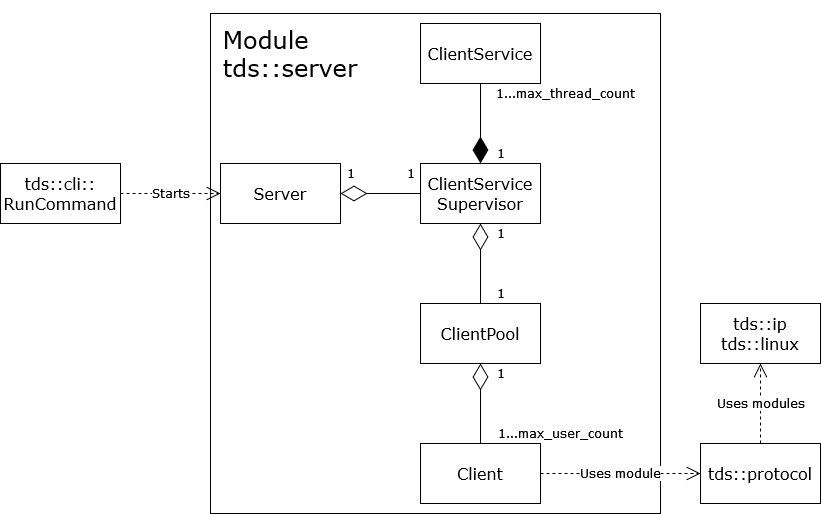
\includegraphics[width=1\textwidth]{img/server-com.png}
\caption{\label{fig:server-com.png}Schemat komunikacji z głównym modułem}
\end{figure}
\FloatBarrier

\pagebreak
\subsubsection{Tryby pracy klienta}
Dla każdego podłączonego klienta klasa \texttt{tds::server::ClientPool} tworzy instancję klasy \texttt{tds::server::Client}, która zawiera podstawowe obiekty potrzebne do przeprowadzenia komunikacji z klientem, czyli między innymi gniazdo, interpreter protokołu czy menadżera pobierania plików. Zasadniczo klasa ta jest automatem skończonym o następujących stanach:
\begin{figure}[ht]
\centering
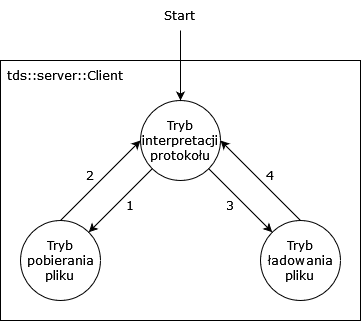
\includegraphics[width=0.5\textwidth]{img/server-cstates.png}
\caption{\label{fig:server-cstates.png}Schemat przechodzenia między trybami klienta}
\end{figure}
\FloatBarrier
\noindent Opis trybów pracy:
\begin{enumerate}
    \item Tryb interpretacji protokołu -- w tym trybie wszystkie dane wejściowe traktowane są jako fragmenty poleceń. Są one przekazywane do interpretera poleceń (instancja klasy \quotcode{tds::protocol::ProtocolInterpreter}), który w momencie wczytania pełnego polecenia próbuje utworzyć obiekt klasy \quotcode{tds::protocol::Request} i przekazuje go do wykonawcy komend (\quotcode{tds::protocol::DefaultCommandExecutor}).
    \item Tryb pobierania pliku -- w tym trybie dane wejściowe są zablokowane. Instancja obsługująca klienta wykorzystując menadżera pobierania (obiekt klasy \quotcode{DownloadManager}) wysyła dane w najwydajniejszy możliwy sposób bezpośrednio do klienta.
    \item Tryb ładowania pliku -- w tym trybie wszystkie dane wejściowe są traktowane jako fragmenty pliku. Instancja obsługująca klienta wykorzystując menadżera ładowania (obiekt klasy \quotcode{UploadManager}) tworzy plik i monitoruje status operacji.
\end{enumerate}
\noindent Przejścia w schemacie:
\begin{enumerate}
    \item Przejście w tryb pobierania pliku -- jest to możliwe tylko w przypadku wykonania polecenia \quotcode{dls} przez klienta.
    \item Przejście z trybu pobierania do trybu interpretacji -- następuje automatycznie po przeczytaniu przez klienta wszystkich bajtów pobieranego pliku.
    \item Przejście w tryb ładowania pliku -- jest to możliwe tylko w przypadku pozytywnego wykonania polecenia \quotcode{ul} przez klienta.
    \item Przejście z trybu ładowania do trybu interpretacji -- następuje automatycznie po wczytaniu przez serwer wszystkich bajtów pliku.
\end{enumerate}

\subsection{Narzędzia i biblioteki}
\subsubsection{Narzędzia}
\bgroup
    \begin{center}
        \def\arraystretch{1.3}
        \begin{tabular}{c|c|c}
            \textbf{Element} & \textbf{Narzędzia} & \textbf{Wersja} \\
            \hline
            Język programowania & \texttt{C++} & ISO/IEC 14882:2020 \\
            \hline
            Kompilator & \makecell{\texttt{g++} \\ \texttt{clang}} & \makecell{11.1.0 \\ 13.0.0} \\
            \hline
            System budowania & \texttt{\href{https://cmake.org/}{CMake}} & \makecell{3.18.4} \\
            \hline
            Automatyzacja testów & \texttt{CTest} & \makecell{3.18.4} \\
            \hline
            Platforma docelowa & \texttt{Linux x86-64} & 4.0 -- 5.16
        \end{tabular}
    \end{center}
\egroup
\subsubsection{Biblioteki}
\bgroup
    \begin{center}
        \def\arraystretch{1.3}
        \begin{tabular}{c|c|c}
            \textbf{Nazwa} & \textbf{Wersja} & \textbf{Opis} \\
            \hline
            \texttt{\href{https://github.com/catchorg/Catch2}{Catch2}} & 3.0.0 & Tworzenie testów jednostkowych \\
            \hline
            \texttt{\href{https://github.com/marzer/tomlplusplus}{tomlplusplus}} & 2.5.0 & Obsługa formatu TOML \\
            \hline
            \texttt{\href{https://github.com/fmtlib/fmt}{\{fmt\}}} & 8.0 & \makecell{Formatowanie tekstów\\(Odpowiednik \texttt{std::format} z C++20)} \\
            \hline
            \texttt{\href{https://github.com/gabime/spdlog}{spdlog}} & 1.9 & \makecell{Tworzenie logów\\(Używane przez klasy z modułu \texttt{tds::server})} \\
        \end{tabular}
    \end{center}
\egroup

\section{Klient mobilny}

\subsection{Opis klienta}
Połączenie z serwerem za pomocą klienta w aplikacji mobilnej zaimplementowane z użyciem języka kotlin w środowisku Android Studio. Za ich pomocą powstanie prosta aplikacja mobilna z interakcyjnym interfejsem graficznym reprezentująca nasz zdalny system plików. Aplikacja będzie budowana na system Android.

\subsection{Narzędzia i biblioteki}
\bgroup
    \begin{center}
        \def\arraystretch{1.3}
        \begin{tabular}{c|c}
            \textbf{Element} & \textbf{Narzędzia} \\
            \hline
            Język programowania & \texttt{Kotlin} \\
            \hline
            Kompilator & \texttt{kotlinc} \\
            \hline
            IDE & \texttt{Android Studio} \\
            \hline
            Platforma docelowa & \texttt{Android}
        \end{tabular}
    \end{center}
\egroup

\section{Klient okienkowy}

\subsection{Opis klienta}
Połączenie z serwerem realizowane przez klienta okienkowego zaimplementowanego z użyciem języka Java i klasy Socket, która reprezentuje gniazda klienckie. Po uruchomieniu klient podejmie próbę połączenia z serwerem. W przypadku udanego połączenia aplikacja umożliwi interakcję ze zdalnym systemem plików.

\subsection{Narzędzia i biblioteki}
\bgroup
    \begin{center}
        \def\arraystretch{1.3}
        \begin{tabular}{c|c}
            \textbf{Element} & \textbf{  Narzędzia  } \\
            \hline
            Język programowania & \texttt{Java}  \\
            \hline
            Kompilator & \texttt{javac} \\
            \hline
            Testy jednostkowe & \texttt{JUnit}  \\
            \hline
            System budowania & \texttt{Gradle}  \\
        \end{tabular}
    \end{center}
\egroup

\section{Klient konsolowy}

\subsection{Opis klienta}
Połączenie z serwerem realizowane poprzez klienta zaimplementowanego przy użyciu biblioteki \texttt{FTXUI} i języka \texttt{C++}. \href{https://github.com/ArthurSonzogni/FTXUI}{FTXUI \textit{(Functional Terminal (X) User interface)}} to biblioteka pozwalająca stworzyć zgrabne TUI. Wykorzystując jej elementy powstanie narzędzie do wykonywania operacji plikowych na zdalnym systemie plików.

Klient konsolowy przeznaczony jest na system \texttt{Ubuntu}. Będzie kompilowany z wykorzystaniem \texttt{g++} oraz budowany z wykorzystaniem \texttt{CMake}.

\subsection{Narzędzia i biblioteki}
\bgroup
    \begin{center}
        \def\arraystretch{1.3}
        \begin{tabular}{c|c|c}
            \textbf{Element} & \textbf{Narzędzia} & \textbf{Wersja} \\
            \hline
            Język programowania & \texttt{C++} & ISO/IEC 14882:2020 \\
            \hline
            Kompilator & \makecell{\texttt{g++}} & \makecell{11.2.0} \\
            \hline
            System budowania & \texttt{\href{https://cmake.org/}{CMake}} & \makecell{3.22.0} \\
            \hline
            TUI & \href{https://github.com/ArthurSonzogni/FTXUI}{\texttt{FTXUI}} & 2.0.0 \\
            \hline
            Platforma docelowa & \texttt{Linux x86-64} & 4.0.0
        \end{tabular}
    \end{center}
\egroup

\pagebreak
\section{Testowanie}

\subsection{Testy jednostkowe}
\subsubsection{Testy serwera}
Testy jednostkowe serwera znajdują się w katalogu \quotcode{server/tests/unit}. Weryfikują one działanie podstawowych modułów systemu takich jak na przykład \quotcode{tds::linux}, który odpowiada za między innymi prawidłowe reagowanie na sygnały systemowe, czy \quotcode{tds::ip}, który odpowiada za nawiązywanie i obsługę połączeń. Ponadto testy te implementują \textit{fuzzing} do sprawdzania działania interpretera poleceń na nieprawidłowe dane wejściowe.

Są to testy automatyczne, można je uruchomić z wykorzystaniem programu \texttt{ctest}: \quotcode{ctest -R UNIT}.

\subsection{Testy integracyjne}
\subsubsection{Testy serwera}
Testy integracyjne znajdują się w katalogu \quotcode{server/tests/integration}. Zostały napisane w języku skryptowym \texttt{Bash}. Ich zadaniem jest sprawdzanie reakcji programu na polecenia linii komend. Ponadto sprawdzana jest prawidłowość wykonania niektórych poleceń klienta z wykorzystaniem programu \texttt{netcat}.

Są to testy automatyczne, można je uruchomić z wykorzystaniem programu \texttt{ctest}: \quotcode{ctest -R INTEGRATION}.

\subsection{Testy penetracyjne}
Testy penetracyjne serwera są wykonywane manualnie. Zakładamy, że osoba atakująca serwer będzie próbowała wykonować następujące akcje:
\begin{enumerate}
    \item Atakujący próbuje dostać się do katalogów zabronionych, czyli takich do których dostęp powinien mieć tylko właściciel serwera, z wykorzystaniem polecenia \quotcode{cd}. Serwer powinien w takim przypadku zawsze skierować użytkownika do katalogu głównego.
    \item Atakujący wysyła losowe ciągi bajtów w celu doprowadzenia do błędu interpretera. W takiej sytuacji moduł odpowiadający za obsługę klienta powinien zadbać o to, aby interpreter nie znalazł się w stanie niedozwolonym (np. nie powinien wpaść w pętlę nieskończoną).
    \item Atakujący wysyła wiele prawidłowych poleceń na raz. W takiej sytuacji serwer powinien wysłać wiele odpowiedzi w jednym momencie oraz nie powinien dopuścić do nadmiernej alokacji pamięci na przyjęte dane.
\end{enumerate}

\subsection{Testy empiryczne}
\noindent Testy manualne wykonywane w ramach testów empirycznych:
\begin{enumerate}
    \item Zweryfikowanie reakcji serwera na nieistniejące lub nieprawidłowo sformułowane polecenia z wykorzystaniem programu \texttt{netcat},
    \item Zweryfikowanie wszystkich poleceń serwera z wykorzystaniem programu \texttt{netcat},
    \item Wykonanie wszystkich poleceń z wykorzystaniem każdego klienta z osobna,
    \item Przetestowanie poprawności obsługi wszystkich scenariuszy alternatywnych dla poleceń,
    \item Sprawdzenie pobierania plików o różnych rozmiarach (od kilku kilobajtów do dwóch gigabajtów),
    \item Sprawdzenie ładowania plików o różnych rozmiarach,
    \item Przerywanie połączenia w trakcie ładowania lub pobierania, oraz wznawianie tych operacji.
\end{enumerate}

\section{Zespół}

\subsection{Środowisko deweloperskie}

\bgroup
    \begin{center}
        \def\arraystretch{1.3}
        \begin{tabular}{c|c|c}
            \textbf{Element} & \textbf{Narzędzia} & \textbf{Wersja} \\
            \hline
            System operacyjny & \texttt{\makecell{Ubuntu \\ Manjaro Linux \\ Windows \\ Arch Linux}} & \makecell{20.04, 21.10 \\ 21.1.6 \\ 10.0 \\ ---} \\
            \hline
            \makecell{Pomocniczy język \\ skryptowy\footnotemark[1]} & \texttt{Bash} & 5.1.8 \\
            \hline
            Kontrola wersji & \texttt{git} & 2.32.0 \\
            \hline
            \makecell{Repozytorium \\ ITS\footnotemark[2] \\ Tablica kanban} & \texttt{\makecell{\href{https://github.com/JMazurkiewicz/TIN-project}{GitHub} \\ \href{https://github.com/JMazurkiewicz/TinDox/issues}{GitHub Issues} \\ \href{https://github.com/JMazurkiewicz/TinDox/projects/1}{GitHub Projects}}} & --- \\
            \hline
            CI/CD & \texttt{Github Actions} & --- \\
            \hline
            Dokumentacja & \texttt{\href{https://www.overleaf.com/read/knbjwfrmvhzq}{Overleaf}} & --- \\
        \end{tabular}
    \end{center}
\egroup
\footnotetext[1]{Języki skryptowe będą używane do np. symulowania złożonych przypadków testowych, automatyzacji testów.}
\footnotetext[2]{Issue tracking system.}

\subsection{Podział pracy}

\begin{center}
    \begin{tabular}{l|r}
        \textbf{Projekt} & \textbf{Wykonawca} \\
        \hline
        Serwer & Jakub Mazurkiewicz \\
        Klient mobilny & Damian Piotrowski \\
        Klient okienkowy & Anna Pyrka \\
        Klient konsolowy & Łukasz Reszka
    \end{tabular}
\end{center}

\end{document}
